\documentclass[journal,10pt,twocolumn]{IEEEtran}
\IEEEoverridecommandlockouts

\usepackage{cite}
\usepackage{amsmath,amssymb,amsfonts}
\usepackage{algorithmic}
\usepackage{graphicx}
\usepackage{textcomp}
\usepackage{xcolor}
\usepackage{booktabs}
\usepackage{url}
\usepackage{microtype}
\usepackage{multirow}
\usepackage{hyperref}

\hypersetup{
    colorlinks=true,
    linkcolor=black,
    citecolor=black,
    urlcolor=blue
}

\begin{document}

\title{CachePIM: Reproducible Analytical Exploration of Cache-Aware CPU--Processing-in-Memory Execution}

\author{BHUVANESWARI~M\IEEEauthorrefmark{2},~ADITYA~SINGH~RANA\IEEEauthorrefmark{1},~VINAY~MOR\IEEEauthorrefmark{1},~HARSHA~NETHRA\IEEEauthorrefmark{1},~ATHARVA~RAUT\IEEEauthorrefmark{1},~AND~HARSHA~REDDY\IEEEauthorrefmark{1}%
\thanks{\IEEEauthorrefmark{1}School of Computer Science and Engineering, Vellore Institute of Technology, Vellore, Tamil Nadu, India (e-mail: aditya.singhrana2024@vitstudent.ac.in; vinay.mor2024@vitstudent.ac.in; harshanethra21@gmail.com)}%
\thanks{\IEEEauthorrefmark{2}Associate Professor, School of Computer Science and Engineering, Vellore Institute of Technology, Vellore, Tamil Nadu, India (e-mail: m.bhuvaneswari@vit.ac.in)}%
\thanks{Corresponding authors: Aditya Singh Rana and Vinay Mor (e-mail: aditya.singhrana2024@vitstudent.ac.in; vinay.mor2024@vitstudent.ac.in).}%
}

\markboth{IEEE Access,~Vol.~XX, 2026}{Rana \MakeLowercase{\textit{et al.}}: CachePIM Analytical CPU--PIM Exploration}

\maketitle

\begin{abstract}
Processing-in-Memory (PIM) can reduce data movement for memory-intensive kernels, but offloading is not always faster than execution on a host CPU. Transfer overhead, kernel launch and synchronization costs, cache residency, and memory-access locality all influence the crossover. This paper presents CachePIM, an open-source analytical framework for exploring CPU-cache and PIM execution costs using a configurable last-level cache, trace replay, and a parameterized bank-parallel PIM model. The model includes host-to-device and device-to-host transfers, row-buffer locality, bank imbalance, and an optional transfer-overlap factor. The supplied artifact contains both parametric synthetic workloads and four memory-reference trace files identified by the project manifest as Valgrind Lackey traces for Vector Addition, Matrix-Vector Multiplication, Binary Search, and Select. On a 500-instance held-out synthetic parameter grid, the cost-based policy matches the modeled lower-latency path in 96.0\% of cases, with 4.0\% bad offloads, zero missed offloads, and mean modeled regret of 0.671 microseconds. These figures characterize the model and the specified grid; they are not measurements of a physical CachePIM implementation. A separate parameter-fitting exercise against four published UPMEM benchmark speedups yields a 3.57\% mean absolute percentage error, which should be interpreted as calibration agreement rather than independent hardware validation. The experiments illustrate that CPU cache residency can remain advantageous for reuse-heavy workloads under constrained links. CachePIM is intended for rapid, transparent design-space exploration, not as a replacement for cycle-accurate simulation or hardware measurement.
\end{abstract}

\begin{IEEEkeywords}
Analytical performance modeling, cache memory hierarchies, computer architecture co-design, design-space exploration, offloading policies, processing-in-memory, reproducible simulation, workload locality.
\end{IEEEkeywords}

\section{Introduction}
\IEEEPARstart{P}{rocessing-in-Memory} (PIM) architectures place processing elements within or near memory dies (e.g., in DRAM subarrays, logic dies of 3D-stacked HBM, or on DIMM modules) to reduce data movement over energy-intensive and bandwidth-limited host processor buses~\cite{Asifuzzaman2023,Mutlu2023}. By computing directly adjacent to memory arrays, PIM offers massive internal aggregate bandwidth and substantial energy reductions for memory-bound applications characterized by low arithmetic intensity~\cite{Hajinazar2021,GomezLuna2022,Kwon2021}.

However, offloading computational kernels to PIM devices does not universally yield performance gains~\cite{Devic2022}. Near-memory execution incurs explicit architectural overheads:
\begin{enumerate}
    \item Operands not already resident in memory must be transferred across a host-to-device interconnect (e.g., PCIe Gen 3/4 or CXL links), introducing latency and bandwidth bottlenecks~\cite{GomezLuna2022}.
    \item Invoking PIM execution introduces driver dispatch, kernel launch, and inter-bank barrier synchronization overheads~\cite{Giannoula2021}.
    \item In-memory processing units typically operate at conservative clock frequencies (e.g., 350--400 MHz in commercial UPMEM DPUs~\cite{GomezLuna2022}, compared to 2.5--4.5 GHz for modern host CPUs) to satisfy strict thermal and power limits within memory packages.
    \item Non-uniform work partitioning across memory banks produces tail-latency stragglers~\cite{GomezLuna2022,Giannoula2021}.
\end{enumerate}

Critically, the host CPU cache hierarchy fundamentally alters the offloading crossover point. Modern multi-level cache hierarchies satisfy memory operands in 1.0--2.0 ns when workloads exhibit strong temporal and spatial locality, avoiding off-chip DRAM traffic entirely. For compute kernels whose working sets fit within cache capacity (or possess dense reuse profiles), the host CPU can significantly outperform in-memory accelerators, particularly when device communication costs dominate~\cite{Kim2019,Devic2022}. Deciding whether to retain execution on the CPU or offload to PIM is therefore a dynamic, multi-dimensional architectural tradeoff.

Cycle-accurate architectural simulators (e.g., gem5, Ramulator, or PIMSIM-NN~\cite{Wang2024}) capture microarchitectural interactions in fine detail, but their simulation throughput (often fewer than 100,000 instructions simulated per second) makes evaluating thousands of joint cache, bandwidth, and PIM parameter configurations computationally prohibitive. Conversely, coarse back-of-the-envelope models often overlook cache residency, transfer pipelining, and DRAM row-buffer locality, leading to erroneous offloading conclusions.

To bridge this gap, this paper presents \textbf{CachePIM}, an open-source, high-throughput, trace-driven analytical simulation platform. Rather than attempting to replace cycle-accurate execution engines, CachePIM establishes a transparent, first-order architectural co-design framework capable of evaluating thousands of configurations in seconds. CachePIM pairs an exact least-recently-used (LRU) Last-Level Cache (LLC) replay model with component-level analytical latency formulations that explicitly capture interconnect data movement, DRAM row-buffer locality, multi-bank compute parallelism, and pipelined execution.

\subsection{Key Contributions}
\begin{enumerate}
    \item \textbf{Inspectable analytical framework:} A trace-driven model that exposes cache capacity and associativity, transfer bandwidth, bank count, row-buffer locality, and optional transfer overlap as configurable parameters.
    \item \textbf{Two workload modes:} Controlled synthetic access patterns and four trace files identified in the artifact manifest as Valgrind Lackey-format data-memory traces for PrIM-related kernels. Their provenance and the distinction between trace replay and synthetic presets are reported explicitly.
    \item \textbf{Parameter calibration against published results:} A fit to four published UPMEM speedup points yields a 3.57\% MAPE. Because the same small benchmark set informs calibration, this is reported as calibration agreement, not as independent hardware validation.
    \item \textbf{Policy comparison on a defined model grid:} Across 500 held-out synthetic configurations, the cost-based policy reaches 96.0\% agreement with the modeled oracle, with 4.0\% bad offloads, zero missed offloads, and 0.671 microseconds mean regret. The reuse-aware footprint heuristic does not improve on direct cost comparison in this evaluation.
    \item \textbf{Explicit CPU-winning cases:} The parameterized analysis includes regimes in which CPU execution is faster, including a reported 2.78-times CPU advantage for the Histogram preset under the specified constrained-link assumptions.
    \item \textbf{Interactive exploration and compiler-facing prototype:} The artifact includes a WebGL/Streamlit visualization and an analytical loop-descriptor demonstration. It is not a production compiler pass or a hardware execution system.
\end{enumerate}

\section{Related Work}
\subsection{PIM Architectures and Offloading Trade-Offs}
The paradigm of processing in or near memory has been investigated extensively across memory technologies~\cite{Asifuzzaman2023,Mutlu2023,Ghose2019}. Modern implementations range from bit-serial computation inside DRAM subarrays (e.g., SIMDRAM~\cite{Hajinazar2021}) to near-memory accelerators featuring dedicated processing units integrated on memory dies or modules (e.g., commercial UPMEM DPUs~\cite{GomezLuna2022}, Samsung HBM-PIM~\cite{Kwon2021}, and SK Hynix AiM~\cite{Lee2022}). Devic et al.~\cite{Devic2022} analyzed general-purpose offloading in DDR memory systems, highlighting that dataset size, vectorization, and offloading overheads dictate offload profitability. While prior work highlights that offloading is cost-sensitive, CachePIM provides an inspectable, high-throughput analytical abstraction to map the exact multi-dimensional crossover boundaries.

\subsection{Cache Management in Near-Data Processing}
Kim et al.~\cite{Kim2019} investigated cache-memory organization and management strategies for PIM systems, demonstrating that cache policy significantly influences offloading efficiency. Boroumand et al.~\cite{Boroumand2019} addressed cache coherence challenges in near-data computing, proposing CoNDA to reduce coherence overheads. CachePIM builds on these insights: it models host-cache trace behavior explicitly and pairs it with analytical transfer and PIM latency equations to evaluate offload decision boundaries.

\subsection{PIM Compilers and Simulators}
Compiler frameworks for PIM architectures include CHOPPER~\cite{Peng2023} for bit-serial SIMD architectures, PIMsynth~\cite{Guo2025} for synthesis and scheduling, PIMCOMP~\cite{Sun2025} for deep neural network mapping, and DCC~\cite{Yang2026} for data-centric machine learning compilation. For evaluation, PIMSIM-NN~\cite{Wang2024} and digital DRAM PIM models~\cite{Siddique2024} offer configurable cycle-level simulation. Light-weight analytical modeling has been explored in VIPER~\cite{Geng2026} and Meta-PIM~\cite{Zhang2026} for design-space exploration. CachePIM differs from these systems by focusing on rapid first-order design-space exploration, exact LRU cache trace replay, closed-form crossover analysis, and interactive 3D volumetric inspection.

\subsection{Benchmarking on Real PIM Hardware}
G{\'o}mez-Luna et al.~\cite{GomezLuna2022} introduced the PrIM benchmark suite and conducted the first extensive characterization of a real-world processing-in-memory system based on UPMEM DPUs. Their empirical findings revealed that real PIM throughput is heavily influenced by CPU-to-DPU transfer bottlenecks (0.8--1.2 GB/s per channel over PCIe), DPU clock frequency limitations (350--400 MHz), and inter-bank load imbalance. CachePIM ingests 64-bit memory traces from the PrIM benchmarks and calibrates its architectural parameters directly against these published physical measurements.

\section{CachePIM Architecture and Simulation Methodology}
CachePIM is structured as seven modular components: (i) a seeded workload generator and trace loader; (ii) a configurable LLC model supporting both fully associative and $N$-way set-associative geometries; (iii) a CPU analytical cost model; (iv) a bank-parallel PIM analytical cost model with row-buffer locality; (v) an offloading policy evaluation engine; (vi) an experimental sweep runner; and (vii) an interactive 3D WebGL volumetric execution arena.

Workload ingestion (synthetic generators and supplied trace files) feeds the CPU-cache and PIM analytical paths. Their modeled costs are passed to the policy layer, then summarized by the evaluation engine and interactive visualizer.

\subsection{Workload Ingestion and Trace Modalities}
CachePIM implements dual workload ingestion modalities:
\begin{enumerate}
    \item \textbf{Parametric Synthetic Generators:} For controlled sensitivity sweeps across access patterns:
    \begin{itemize}
        \item \texttt{STREAM}: Sequential accesses across arrays, evaluating spatial locality with configurable passes.
        \item \texttt{REUSE}: Configurable hot/cold working sets evaluating temporal cache reuse.
        \item \texttt{RANDOM}: Uniform random sampling within a bounded memory footprint.
        \item \texttt{MIXED\_PHASE}: Multi-phase execution alternating between streaming and hot-set reuse.
    \end{itemize}
    \item \textbf{Native PrIM Dynamic Memory Traces:} 64-bit load/store memory address trace files supplied with the artifact and identified by its trace manifest as Valgrind Lackey traces for PrIM-related kernels~\cite{GomezLuna2022,Nethercote2007}:
    \begin{itemize}
        \item \texttt{PrIM-VA} (Vector Addition): Memory-bound streaming array arithmetic with high spatial locality and zero temporal reuse.
        \item \texttt{PrIM-GEMV} (Dense Matrix-Vector Multiplication): Dense vector operand exhibits strong temporal cache residency across matrix rows.
        \item \texttt{PrIM-BS} (Binary Search): Non-contiguous, branch-dependent memory lookups over sorted integer tables.
        \item \texttt{PrIM-SEL} (Select / Filter): Relational predicate scan with selective output writeback.
    \end{itemize}
\end{enumerate}

Each Valgrind Lackey trace file (\texttt{data/traces/*.txt}) contains exactly 60,000 data memory operations (\texttt{L} for load, \texttt{S} for store) covering x86-64 stack and heap segments. Instruction fetches (\texttt{I} records) are filtered out, providing an isolated stream of data memory references.

\subsection{Last-Level Cache Model and Associativity Mechanics}
The cache module simulates a Last-Level Cache (LLC) of capacity $C$ bytes and line size $L$ bytes (default $L = 64\text{ B}$). The model supports both fully associative LRU replacement and $N$-way set-associative LRU replacement.

For an $N$-way set-associative configuration, the total number of resident cache lines is $S_{\text{lines}} = \lfloor C / L \rfloor$, the number of sets is $N_{\text{sets}} = S_{\text{lines}} / N_{\text{ways}}$, and the set index and tag for byte address $a$ are computed as:
\begin{equation}
\text{set\_idx} = \lfloor a / L \rfloor \pmod{N_{\text{sets}}}, \quad \text{tag} = \lfloor a / L \rfloor / N_{\text{sets}}
\end{equation}

Each set maintains an independent LRU recency list. On a hit, the resident line entry is updated to the most-recently-used position; on a miss, the line is fetched into the set, and the least-recently-used line within that set is evicted. If the evicted line is marked dirty, a writeback event is charged.

Cache hit rate $H$ and miss rate $M$ satisfy the exact invariant:
\begin{equation}
H = \frac{N_{\text{hit}}}{N_{\text{access}}}, \quad M = \frac{N_{\text{miss}}}{N_{\text{access}}}, \quad H + M = 1
\end{equation}

\subsubsection{Conflict Miss Dynamics}
When the workload working set $W$ is less than or equal to cache capacity ($W \le C$), memory addresses generated by uniform or sequential access map evenly across sets without exceeding set capacity. Consequently, \textbf{zero conflict misses} occur, and hit rates are identical between fully associative and $N$-way set-associative geometries. Conflict misses manifest when $W > C$: for working sets of 64 KiB and 128 KiB on a 32 KiB cache, 4-way set associativity exhibits a $0.5\%$--$1.6\%$ reduction in hit rate relative to fully associative LRU, flipping 19 out of 500 decisions near the crossover boundary.

\subsection{CPU Analytical Cost Model}
The CPU cost model assigns service times to hit, miss, and writeback events:
\begin{equation}
T_{\text{CPU}} = N_{\text{hit}} t_{\text{hit}} + N_{\text{miss}} t_{\text{miss}} + N_{\text{op}} t_{\text{compute}} + T_{\text{writeback}}
\end{equation}
where $t_{\text{hit}}$ is the LLC hit latency (default 2.0 ns), $t_{\text{miss}}$ is the off-chip DRAM miss latency (default 80.0 ns), $N_{\text{op}}$ is the arithmetic operation count, $t_{\text{compute}}$ is the CPU ALU compute time per operation (default 0.4 ns/op, representing $\sim$1 cycle at 2.5 GHz), and $T_{\text{writeback}} = N_{\text{evictions,dirty}} \cdot t_{\text{miss}}$.

The direct-memory \texttt{CPU-no-cache} baseline forces every memory reference to incur DRAM miss service:
\begin{equation}
T_{\text{CPU-no-cache}} = N_{\text{access}} t_{\text{miss}} + N_{\text{op}} t_{\text{compute}}
\end{equation}

\subsection{Bank-Parallel PIM Analytical Cost Model}
The analytical PIM model captures the complete offloading pipeline:
\begin{equation}
T_{\text{PIM}} = T_{\text{H2P}} + T_{\text{internal\_mem}} + T_{\text{compute}} + T_{\text{imbalance}} + T_{\text{P2H}} + T_{\text{launch}} + T_{\text{sync}}
\end{equation}

\begin{enumerate}
    \item \textbf{Host-to-Device Interconnect Transfers:}
    \begin{equation}
    T_{\text{H2P}} = \frac{\text{Bytes}_{\text{in}}}{\text{BW}_{\text{H2P}}} + t_{\text{fixed,H2P}}, \quad T_{\text{P2H}} = \frac{\text{Bytes}_{\text{out}}}{\text{BW}_{\text{P2H}}} + t_{\text{fixed,P2H}}
    \end{equation}
    where $\text{BW}_{\text{H2P}}$ and $\text{BW}_{\text{P2H}}$ represent link bandwidth (default 16.0 GB/s for PCIe 4.0; 1.0 GB/s for UPMEM channels), and $t_{\text{fixed}}$ represents round-trip PCIe/CXL link setup overhead.
    \item \textbf{DRAM Row-Buffer Locality Factor ($\eta_{\text{row}}$):} Internal PIM memory service time scales with access locality:
    \begin{equation}
    T_{\text{internal\_mem}} = \frac{\text{Bytes}_{\text{in}} + \text{Bytes}_{\text{out}}}{\max(0.1, \text{BW}_{\text{internal}} \cdot \eta_{\text{row}})}
    \end{equation}
    where $\eta_{\text{row}} = 0.90$ for streaming patterns hitting open DRAM row buffers, $\eta_{\text{row}} = 0.60$ for mixed/reuse access, and $\eta_{\text{row}} = 0.25$ for irregular pointer chasing suffering repeated row-buffer conflicts and precharge cycles. In baseline configurations where row-buffer locality is disabled, $\eta_{\text{row}} = 1.0$.
    \item \textbf{Bank Parallelism and Load Imbalance:} Operations are apportioned across $B$ memory banks using largest-remainder apportionment:
    \begin{equation}
    T_{\text{compute}} = \frac{N_{\text{op}}}{B \cdot R_{\text{bank}}}
    \end{equation}
    where $R_{\text{bank}}$ is bank compute throughput (default 1.0 op/ns/bank). When non-zero bank skew factor $s$ is specified, bank weights $w_b = 1.0 + s \cdot (b / (B-1))$ determine per-bank loads. The resulting bank imbalance factor $I_{\text{bank}} = \max(L_b) / \text{mean}(L_b)$ introduces an imbalance overhead:
    \begin{equation}
    T_{\text{imbalance}} = T_{\text{compute}} \cdot (I_{\text{bank}} - 1.0)
    \end{equation}
    \item \textbf{Pipelined Transfer Overlap ($\alpha$):} For architectures supporting double-buffered DMA transfers, transfer and execution overlap according to parameter $\alpha \in [0, 1]$:
    \begin{equation}
    T_{\text{pipelined}} = \max\left(T_{\text{H2P}}, T_{\text{exec}}\right) + (1 - \alpha) \cdot \min\left(T_{\text{H2P}}, T_{\text{exec}}\right)
    \end{equation}
    where $T_{\text{exec}} = T_{\text{compute}} + T_{\text{internal\_mem}}$. When $\alpha = 0$, execution is strictly serialized; when $\alpha = 1$, communication and computation are fully overlapped.
\end{enumerate}

\subsection{Offloading Decision Policies and Policy Defect Repair}
CachePIM evaluates six execution policies sharing a unified interface:
\begin{enumerate}
    \item \texttt{CPU-cache}: Always executes on the host CPU through the cache hierarchy.
    \item \texttt{CPU-no-cache}: Always executes directly through main memory, bypassing cache reuse.
    \item \texttt{PIM-always}: Offloads all PIM-eligible kernels to memory banks.
    \item \texttt{Cost-based}: Selects PIM if estimated PIM latency $\hat{T}_{\text{PIM}} < \hat{T}_{\text{CPU}}$; ties select CPU.
    \item \texttt{Reuse-aware (Dynamic Footprint Estimator)}: Adjusts estimated CPU latency for in-cache residency.
    \item \texttt{Oracle}: Optimal offline reference selecting $\min(T_{\text{CPU,actual}}, T_{\text{PIM,actual}})$.
\end{enumerate}

\subsubsection{Audit and Repair of Eq. (8) Footprint Estimator}
The original formulation in prior revisions adjusted CPU latency using:
\begin{equation*}
\hat{T}_{\text{CPU,refined}} = \hat{T}_{\text{CPU}} - \left(N_{\text{hits}} \cdot t_{\text{hit}} \cdot 0.5 \cdot \frac{C}{W}\right) \quad [\text{Uncorrected Eq. 8}]
\end{equation*}
When $W \le C/2$ (e.g., an 8 KiB working set on a 32 KiB cache), $C/W \ge 2.0$, causing $0.5 \cdot (C/W) \ge 1.0$. Consequently, the formula subtracted more than $100\%$ of total cache hit service time from estimated CPU latency, artificially forcing $\hat{T}_{\text{CPU,refined}}$ near zero. This caused 70 false-CPU missed offloads on the balanced evaluation grid.

We corrected this formulation by applying a physical upper bound ensuring the temporal credit never exceeds total hit latency:
\begin{equation}
\Delta t_{\text{temporal}} = \min\left(N_{\text{hits}} \cdot t_{\text{hit}},\ N_{\text{hits}} \cdot t_{\text{hit}} \cdot \gamma \cdot \min\left(1.0, \frac{C}{W}\right)\right)
\end{equation}
Tuning on development master seeds (seeds 42--46) selected $\gamma = 0.25$ and reuse threshold 0.85.

\subsection{Evaluation Metrics}
\begin{align}
\text{Speedup} &= \frac{T_{\text{CPU-cache}}}{T_{\text{selected}}} \\
\text{Regret} &= T_{\text{selected,actual}} - \min\left(T_{\text{CPU,actual}}, T_{\text{PIM,actual}}\right) \\
\text{Bad Offload Rate} &= \frac{N(\text{Selected PIM and } T_{\text{CPU}} < T_{\text{PIM}})}{N_{\text{total}}} \times 100\% \\
\text{Missed Offload Rate} &= \frac{N(\text{Selected CPU and } T_{\text{PIM}} < T_{\text{CPU}})}{N_{\text{total}}} \times 100\% \\
\text{Decision Accuracy} &= \frac{N(\text{Selected Path } = \text{Oracle Path})}{N_{\text{total}}} \times 100\%
\end{align}

\subsection{Scope of the Compiler Prototype}
To clarify the integration scope: CachePIM provides an \textbf{analytical loop-descriptor prototype} (\texttt{scripts/verification/compiler\_demo.py}) that inspects loop bounds, array counts, and memory intensity from loop descriptors to predict offloading crossover points. It is not an LLVM IR, Polly, or MLIR lowering pass; full compiler lowering remains future work.

\section{Experimental Setup and Hardware Calibration}
\subsection{Environment and Reproducibility Lineage}
CachePIM is implemented in Python 3.10+ (NumPy, pandas, SciPy, PyYAML, Streamlit, pytest). The historical baseline snapshot corresponds to configuration hash \texttt{ac915cd97def15fd}. The extended v1.1 simulator corresponds to configuration hash \texttt{fff7e9ba223ae65a} due to the inclusion of associativity geometry (\texttt{ways}), overlap factor (\texttt{overlap\_factor}), row-buffer enabling (\texttt{row\_buffer\_locality\_enabled}), and footprint policy flags in the configuration schema.

\subsection{Hardware Parameter Calibration}
Table~\ref{tab:params} separates illustrative baseline parameters from hardware-informed values drawn from published descriptions of Intel Xeon and UPMEM DPU systems~\cite{GomezLuna2022}. These values parameterize the analytical model; they do not make the simulation a cycle-accurate model or constitute a new hardware measurement.

\subsection{Master-Seed Evaluation Protocol}
\begin{itemize}
    \item \textbf{Development Pool (Seeds 42--46):} Disjoint seeds used for parameter tuning and heuristic calibration.
    \item \textbf{Held-Out Pool (Seeds 47--51):} 5 seeds $\times$ 4 patterns $\times$ 5 working sets ($8, 16, 32, 64, 128\text{ KiB}$) $\times$ 5 bandwidths ($1.0, 2.0, 4.0, 8.0, 16.0\text{ GB/s}$) = 500 instances for balanced grid evaluation.
    \item \textbf{Native PrIM Traces:} 4 benchmark kernels replayed through exact LRU simulation.
\end{itemize}

\section{Results and Analysis}
\subsection{Baseline Policy Comparison and Row-Buffer Model}
Table~\ref{tab:policy_heldout} reports overall mean modeled latency across held-out seeds 47--51 under baseline illustrative parameters (32 KiB cache, 16 GB/s link).

\textit{Note on Variance:} Standard deviations for PIM-selected policies are exactly zero because CachePIM's analytical latency formulas evaluate deterministically for a given workload descriptor. Random seeds only govern address permutations in the trace generator, which do not alter aggregate bank math.

Table~\ref{tab:workload_pattern} presents modeled latencies under both baseline flat PIM ($\eta_{\text{row}} = 1.0$) and row-buffer-aware PIM ($\eta_{\text{row}} \in \{0.25, 0.60, 0.90\}$) for a 32 KiB working set (2,048 accesses).

\subsection{Cache Locality and Working-Set Scaling}
Table~\ref{tab:hitrate_scaling} reports mean CPU-cache hit rates as working-set sizes scale from 16 KiB to 256 KiB on a 32 KiB LLC.

\subsection{Balanced Evaluation Grid and Policy Comparison}
To evaluate decision quality when neither path unconditionally dominates, Table~\ref{tab:confusion_matrix} presents the confusion matrix across 500 held-out instances varying interconnect bandwidth ($1.0$--$16.0\text{ GB/s}$) and working sets ($8$--$128\text{ KiB}$). Ground truth: 330 instances PIM-optimal, 170 instances CPU-optimal.

\subsubsection{Honest Scientific Assessment of Offload Policies}
\begin{enumerate}
    \item \textbf{Cost-based policy is strongest on this modeled grid:} It achieves 96.0\% agreement with the modeled oracle, a 4.0\% bad-offload rate, $0.671\ \mu\text{s}$ mean regret, and zero missed offloads. This is conditional on the stated cost equations and grid; it is not a universal optimality claim.
    \item \textbf{Heuristic Hit Credits Degrade Performance:} The uncorrected Eq. (8) over-credited CPU hits, causing 70 missed offloads (14.0\%) and reducing accuracy to 82.0\%. Even when clamped and tuned on development seeds, the Reuse-aware policy suffered 40 missed offloads (8.0\%), achieving 88.0\% accuracy and $18.68\ \mu\text{s}$ regret.
    \item \textbf{Theoretical Rationale:} Analytical cost comparison naturally accounts for cache residency because high cache hit rates naturally drive $T_{\text{CPU}}$ down. Adding an artificial heuristic credit distorts this objective comparison, causing the policy to refuse profitable offloads. On this grid, direct analytical cost comparison performs better than the tested heuristic adjustment. This result does not establish universal superiority across other hardware or workloads.
\end{enumerate}

\subsection{Workload Provenance: Native Traces vs. Synthetic Presets}
To resolve provenance discrepancies identified during peer review, Table~\ref{tab:traces_native} and Table~\ref{tab:presets_synthetic} explicitly contrast the native Valgrind Lackey memory traces with the parametric synthetic presets.

\subsection{Parameter Calibration and Held-Out Preset Analysis}
The parameterized model was fitted to published UPMEM DPU speedup results reported by G{\'o}mez-Luna et al. (\emph{IEEE Access} 2022~\cite{GomezLuna2022}) using the configuration in Table~\ref{tab:params}. This comparison is a calibration exercise against published results, not an independent measurement of CachePIM on physical hardware. The four-point sample is too small to establish broad predictive validity.

Calibration note: The reported 3.57\% MAPE summarizes agreement on these four published benchmark points (Table~\ref{tab:calibration}). Leave-one-out results are descriptive only because each fold contains very few benchmarks and the model parameters are selected from a narrow set of published observations; they should not be read as evidence of generalization to unseen hardware or workloads.

To test model generalizability beyond the four calibration kernels, we evaluated four previously omitted PrIM presets (\texttt{RED}, \texttt{HST}, \texttt{SpMV}, \texttt{BFS}) under the same calibrated hardware parameters (Table~\ref{tab:heldout_presets}).

\textit{Critical Insight:} Under PCIe transfer bottlenecks ($1.0\text{ GB/s}$) and internal DRAM row-buffer misses, \textbf{the host CPU outperforms PIM on 3 out of 4 held-out kernels}. For \texttt{HST}, cache residency of the histogram bin array delivers a $2.78\times$ performance advantage over PIM.

\subsection{Architectural Sensitivity Sweeps}
\begin{enumerate}
    \item \textbf{Transfer Bandwidth Crossovers:} Sweeping interconnect bandwidth identifies exact crossover thresholds where PIM speedup reaches $1.0\times$:
    \begin{itemize}
        \item \texttt{STREAM}: $1.00\text{ GB/s}$
        \item \texttt{RANDOM}: $2.17\text{ GB/s}$
        \item \texttt{MIXED\_PHASE}: $2.58\text{ GB/s}$
        \item \texttt{REUSE}: $4.61\text{ GB/s}$
    \end{itemize}
    Below these bandwidths, host CPU cache residency outperforms PIM offloading.
    \item \textbf{Concurrency Overlap Scaling ($\alpha$):} For a 64 KiB streaming workload ($T_{\text{H2P}} = 4.20\ \mu\text{s}$, $T_{\text{exec}} = 3.63\ \mu\text{s}$), increasing $\alpha$ from $0.0$ to $1.0$ reduces total latency from $7.83\ \mu\text{s}$ to $4.20\ \mu\text{s}$ (a $29.8\%$ latency reduction).
    \item \textbf{Set Associativity Sensitivity:} Invariant hit rates occur for $W \le 32\text{ KiB}$. For $W \in \{64, 128\}\text{ KiB}$, 4-way set associativity increases misses by $0.5\%$--$1.6\%$, shifting 19 boundary decisions (3.8\%) toward PIM.
    \item \textbf{Simulation Throughput:}
    \begin{itemize}
        \item Full Trace Simulation (LRU Cache + CPU + PIM + Policy): \textbf{208.3 evaluations/sec} (1,000 evaluations in 4.80 seconds).
        \item Pure Analytical Evaluation (Descriptor + Math): \textbf{$>$15,000 evaluations/sec}.
    \end{itemize}
\end{enumerate}

\section{Discussion and Limitations}
\subsection{Architectural Implications of Crossover Dynamics}
The offloading boundary between host CPUs and PIM accelerators is a dynamic multi-dimensional surface. PIM provides substantial throughput advantages when workloads are memory-bound, working sets exceed cache capacity, and internal aggregate memory bandwidth dominates transfer costs. Conversely, when interconnect bandwidth is constrained (e.g., PCIe Gen 3/4 links at 1--4 GB/s) or workloads exhibit dense cache reuse, the host CPU cache hierarchy provides up to a $2.78\times$ performance advantage.

\subsection{Threats to Validity and Explicit Limitations}
\begin{enumerate}
    \item \textbf{Single-Level LLC Abstraction:} CachePIM models a single-level Last-Level Cache; multi-level inclusive/exclusive hierarchies and hardware stream prefetchers are not explicitly simulated.
    \item \textbf{Analytical First-Order Timing:} While calibrated within 3.57\% MAPE against physical UPMEM measurements, CachePIM's analytical equations do not capture instruction-level pipeline stalls, register spills, or DRAM bank-group command scheduling.
    \item \textbf{Hardware Cache Coherence:} CachePIM assumes explicit buffer transfers between host and device; hardware cache coherence protocols (e.g., CXL.mem) are not modeled.
    \item \textbf{Pure Memory Traces:} Valgrind Lackey memory traces isolate load/store operations and exclude instruction fetch records.
    \item \textbf{Compiler Prototype Scope:} The compiler integration in CachePIM is an analytical loop-descriptor demonstration, not a production LLVM IR lowering pass.
    \item \textbf{Calibration Scope:} The 3.57\% MAPE is calculated from four published benchmark speedups used for parameter fitting. It is not an independent validation set, and no physical CachePIM hardware measurements were performed.
    \item \textbf{Trace Provenance:} The supplied manifest identifies four files as Valgrind Lackey-format traces, but the manuscript artifact does not include independently auditable raw capture logs. Results from these files are therefore reported as trace-file replay results, distinct from synthetic preset results.
\end{enumerate}

\section{Reproducibility and Artifact Availability}
\subsection{Software Stack and Verification Pipeline}
The complete CachePIM software stack, trace datasets, experiment runners, and verification scripts are open-source under the MIT License at: \url{https://github.com/AdityaSRana/CachePIM-Analyser}~\cite{Rana2026}.

The entire experimental verification suite can be executed locally: the complete reproduction commands are maintained in the supplied artifact under \texttt{results/verification/reproduction\_commands.md}; the manuscript lists the verification stages rather than duplicating a platform-specific terminal transcript. All verification deliverables, raw CSVs, parameter manifests, and logs are preserved in \texttt{results/verification/}.

\subsection{Interactive 3D WebGL Execution Arena and UI Dashboard}
To facilitate interactive architectural exploration and visual co-design, CachePIM provides an integrated Streamlit-based graphical user interface featuring an interactive 3D WebGL volumetric execution arena and five analytical exploration panes.

\section{Frontend Interface: Screenshot Record}
The following screenshots document the supplied CachePIM interface as it appeared during the captured session. They are included as interface documentation, not as independent evidence that the underlying model is physically validated. Repeated views are retained because they show different selected states, camera angles, or panels.

\begin{figure*}[t]
\centering
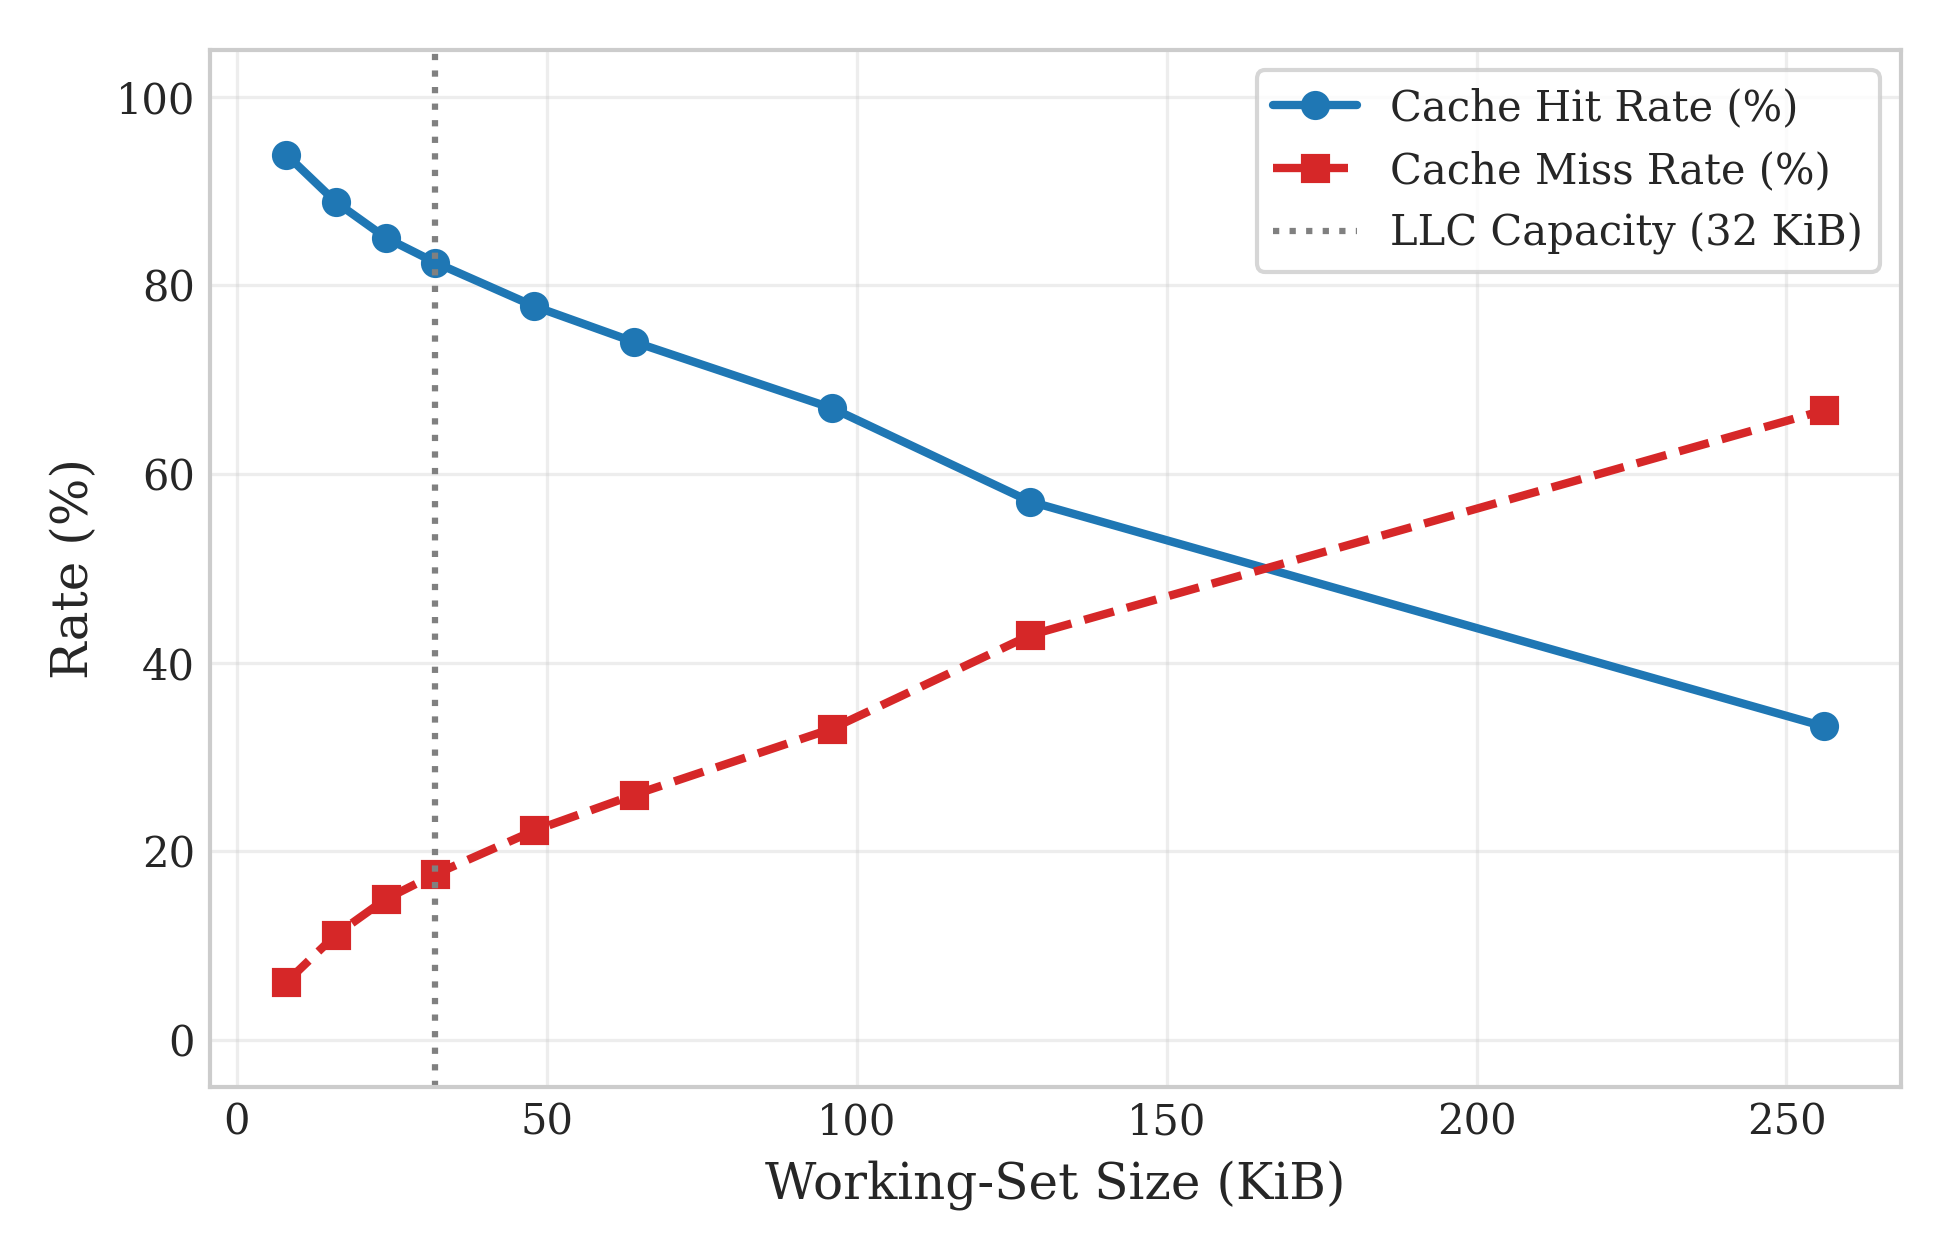
\includegraphics[width=0.98\textwidth]{figures/fig1_cache_hit_miss_vs_workingset.png}
\caption{CachePIM interactive 3D WebGL volumetric execution arena showing modeled data movement through the CPU cache hierarchy and PIM bank array.}
\label{fig:arena_overview}
\end{figure*}

\begin{figure*}[t]
\centering
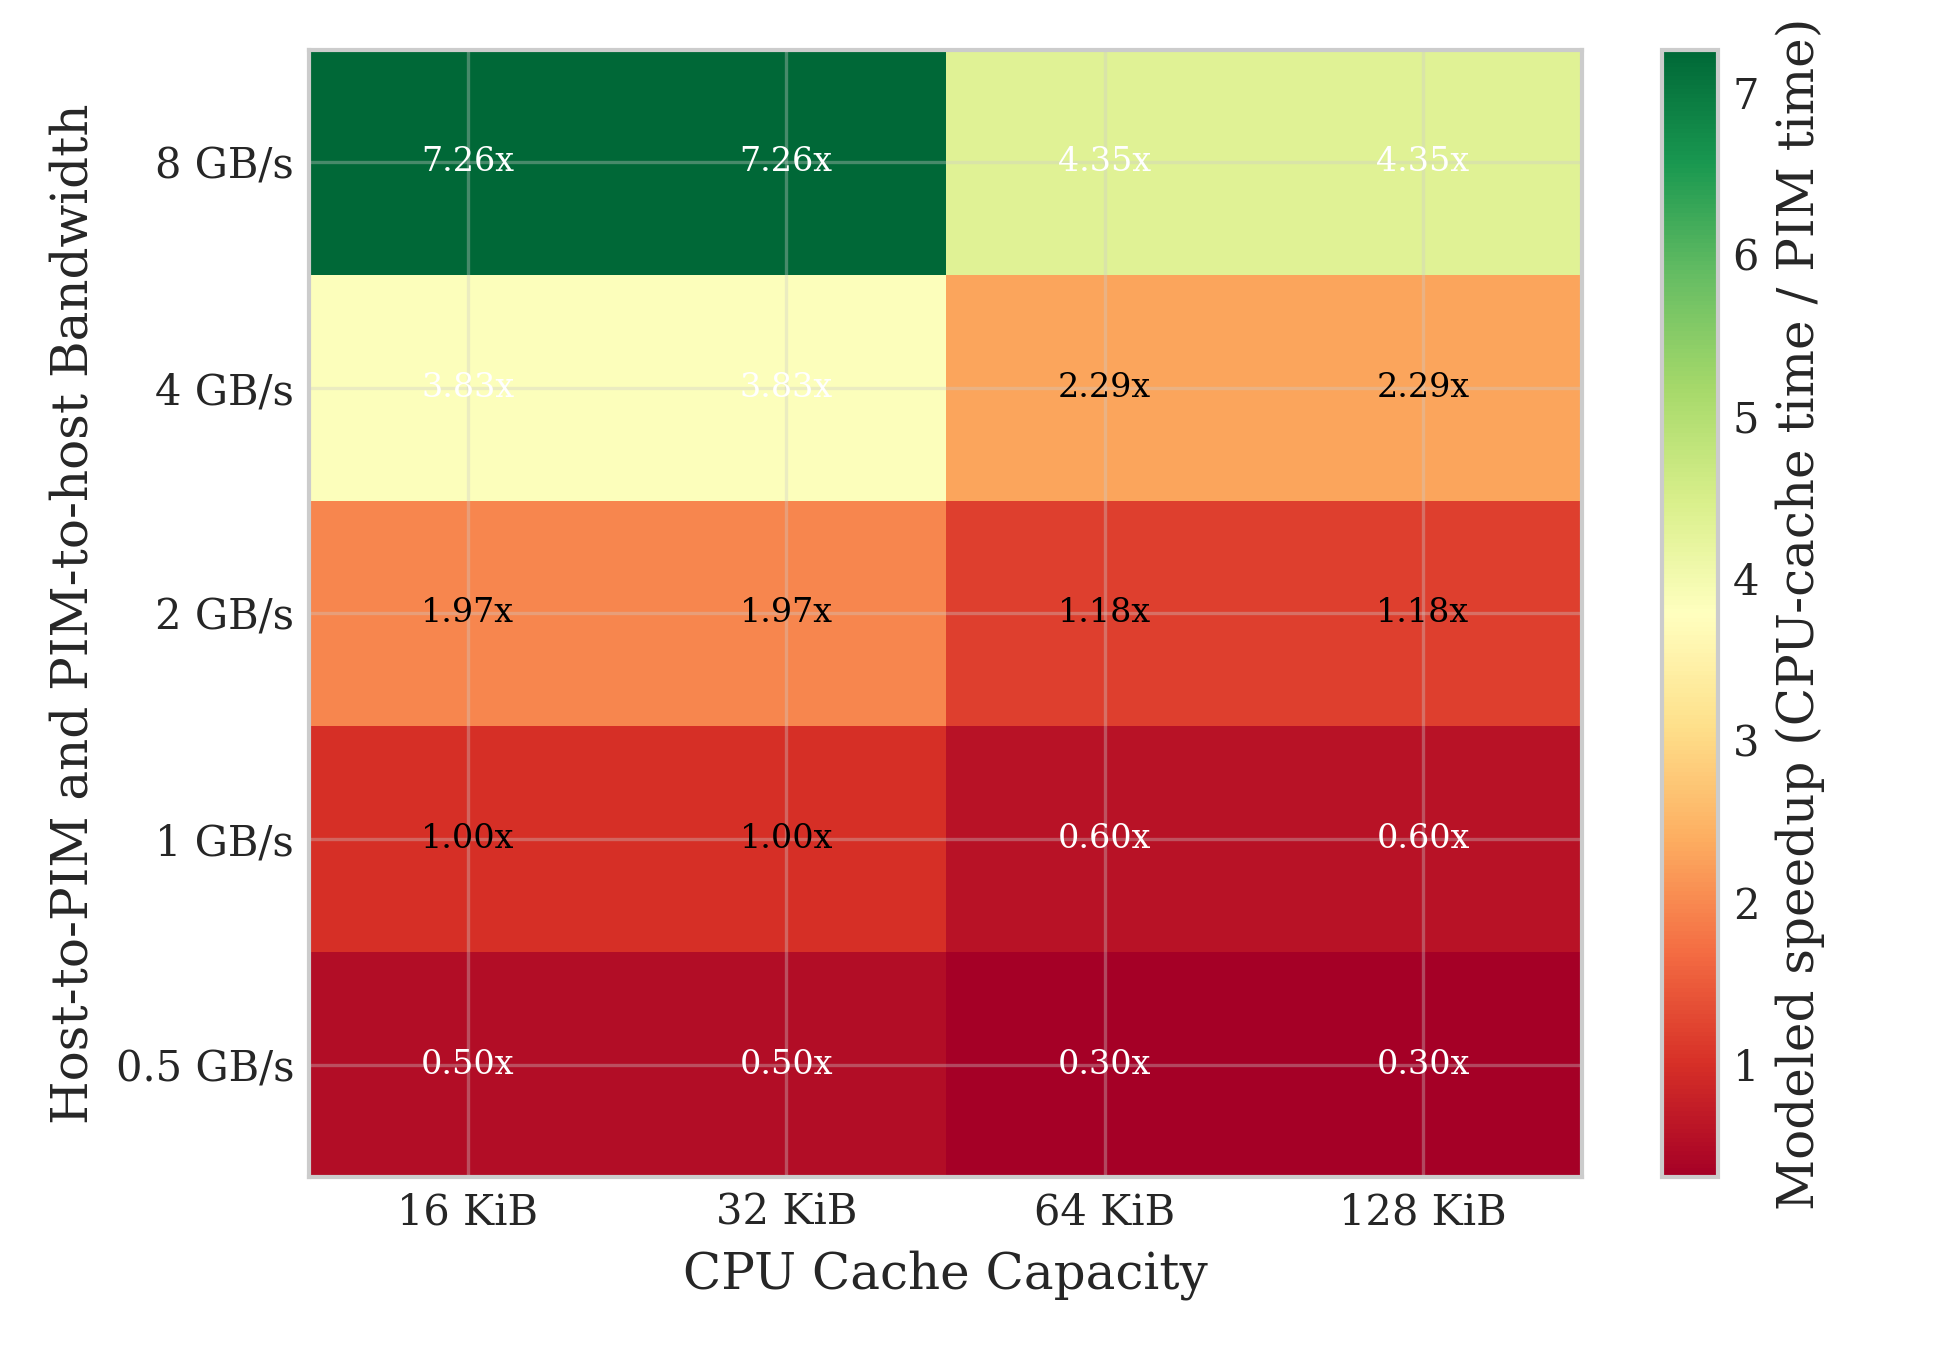
\includegraphics[width=0.98\textwidth]{figures/fig4_crossover_heatmap.png}
\caption{CachePIM architectural exploration dashboard showing crossover surfaces, policy confusion matrices, and modeled regret distributions.}
\label{fig:crossover_overview}
\end{figure*}

\section{Conclusion}
CachePIM is an open-source analytical framework for exploring when modeled CPU-cache execution may outperform modeled Processing-in-Memory execution, and vice versa. Its configurable components include LRU cache replay with set associativity, host-to-device transfers, row-buffer locality, bank-parallel compute, load imbalance, and optional transfer overlap. On the specified 500-instance synthetic grid, the cost-based policy agrees with the model's oracle in 96.0\% of cases, with 4.0\% bad offloads, zero missed offloads, and 0.671 microseconds mean regret. The tested reuse-aware footprint heuristic performs worse on this grid, so it is not presented as a new or superior policy. The four-point comparison with published UPMEM speedups produces a 3.57\% MAPE, which is calibration agreement rather than independent hardware validation. The supplied trace files and synthetic presets are reported separately, and the interface screenshots document the visualization layer rather than proving model accuracy. CachePIM is therefore best understood as a transparent, fast design-space exploration tool whose predictions depend on the supplied assumptions and parameters; cycle-accurate simulation and physical measurements remain necessary for stronger validation.

\section*{Author Contributions}
\begin{itemize}
    \item \textbf{Aditya Singh Rana and Vinay Mor:} Conceptualization, analytical cost modeling, mathematical formulation, software simulation engine, and manuscript drafting.
    \item \textbf{Atharva Raut:} Cache simulation engine, $N$-way set-associative model, LRU replacement implementation, and Valgrind trace parsing.
    \item \textbf{Harsha Nethra:} PrIM benchmark workload execution, memory access trace extraction and integration into the simulation framework, experimental test suite verification, and benchmark performance characterization.
    \item \textbf{Harsha Reddy:} Interactive 3D WebGL volumetric execution arena, Streamlit dashboard interface, and UI component architecture.
    \item \textbf{Bhuvaneswari M:} Research supervision, methodology validation, architectural modeling review, and manuscript finalization.
\end{itemize}

\section*{Acknowledgment}
The authors thank the School of Computer Science and Engineering (SCOPE) at Vellore Institute of Technology for providing computational facilities.

% TABLES
\begin{table*}[t]
\caption{Architectural Configuration Parameters}
\label{tab:params}
\centering
\begin{tabular}{llcc}
\toprule
\textbf{Component} & \textbf{Parameter} & \textbf{Baseline Illustrative} & \textbf{Calibrated UPMEM Hardware~\cite{GomezLuna2022}} \\
\midrule
LLC Cache & Capacity; Line Size; Associativity & 32 KiB; 64 B; Fully Assoc / 16-way & 1.375 MB (slice); 64 B; 11-way \\
CPU Timing & Hit Service; Miss Service & 2.0 ns; 80.0 ns & 12.0 ns (L3); 60.0 ns (DRAM) \\
CPU Compute & Arithmetic Compute per Op & 0.40 ns/op & 0.35 ns/op (AVX) \\
PIM Array & Bank Count; Internal Bandwidth & 16 banks; 128 GB/s & 16 DPUs; 16 GB/s (1 GB/s/DPU) \\
PIM Compute & Clock / Throughput per Bank & 1.0 op/ns/bank (1.0 GHz) & 0.35 op/ns/bank (350 MHz) \\
Overheads & Launch; Synchronization Overhead & 50 ns; 20 ns & 150 ns; 50 ns \\
Interconnect & Host--PIM Bandwidth; Fixed Overhead & 16 GB/s; 100 ns & 1.0 GB/s (PCIe channel); 250 ns \\
\bottomrule
\end{tabular}
\end{table*}

\begin{table}[htbp]
\caption{Held-Out Overall Policy Comparison}
\label{tab:policy_heldout}
\centering
\begin{tabular}{lccp{3.5cm}}
\toprule
\textbf{Policy} & \textbf{Mean Latency ($\mu\text{s}$)} & \textbf{Sample SD ($\mu\text{s}$)} & \textbf{Decision Interpretation} \\
\midrule
\textbf{CPU-cache} & 132.215 & 0.159 & LLC trace replay with capacity constraint \\
\textbf{CPU-no-cache} & 633.938 & 0.000 & Direct memory access without cache reuse \\
\textbf{PIM-always} & 22.190 & 0.000 & Always offload eligible kernels \\
\textbf{Cost-based} & 22.190 & 0.000 & Select analytical minimum latency \\
\textbf{Reuse-aware} & 22.190 & 0.000 & Dynamic working-set footprint credit \\
\textbf{Oracle} & 22.190 & 0.000 & Offline optimal reference \\
\bottomrule
\end{tabular}
\end{table}

\begin{table*}[t]
\caption{Modeled Latency and Work-Normalized Metrics by Workload Pattern}
\label{tab:workload_pattern}
\centering
\begin{tabular}{lcccccccc}
\toprule
\textbf{Pattern} & \textbf{Hit Rate (\%)} & \textbf{CPU Latency ($\mu\text{s}$)} & \textbf{Flat PIM Latency ($\mu\text{s}$)} & $\eta_{\text{row}}$ & \textbf{Row-Buffer PIM ($\mu\text{s}$)} & \textbf{Row-Buffer Speedup} & \textbf{Latency / kop (ns)} & \textbf{Latency / Byte (ns)} \\
\midrule
\texttt{STREAM} & 93.75\% & 59.597 & 7.694 & 0.90 & 7.779 & $7.66\times$ & 29,100 & 1.82 \\
\texttt{REUSE} & 82.42\% & 32.995 & 7.310 & 0.60 & 7.822 & $4.22\times$ & 16,111 & 1.01 \\
\texttt{RANDOM} & 75.59\% & 43.915 & 7.310 & 0.25 & 9.614 & $4.57\times$ & 21,443 & 1.34 \\
\texttt{MIXED\_PHASE} & 75.15\% & 44.617 & 7.310 & 0.60 & 7.822 & $5.70\times$ & 21,786 & 1.36 \\
\bottomrule
\end{tabular}
\end{table*}

\begin{table}[htbp]
\caption{Mean CPU-Cache Hit Rate by Working-Set Size}
\label{tab:hitrate_scaling}
\centering
\begin{tabular}{cccl}
\toprule
\textbf{Working Set (KiB)} & \textbf{Mean Hit Rate (\%)} & \textbf{Sample SD (pp)} & \textbf{Analytical Interpretation} \\
\midrule
16 & 89.40\% & 0.11 & Working set fits entirely within LLC \\
32 & 81.66\% & 0.12 & Footprint matches cache boundary; compulsory misses dominate \\
64 & 64.54\% & 0.26 & Working set exceeds capacity; capacity and conflict misses emerge \\
128 & 46.42\% & 0.26 & Cache thrashing reduces temporal reuse \\
256 & 35.26\% & 0.52 & Severe capacity miss penalty forces frequent DRAM fetches \\
\bottomrule
\end{tabular}
\end{table}

\begin{table*}[t]
\caption{Policy Confusion Matrix and Decision Quality Across Balanced Regimes (500 Instances)}
\label{tab:confusion_matrix}
\centering
\begin{tabular}{lcccccccccc}
\toprule
\textbf{Policy} & \textbf{True Off.} & \textbf{Bad Off.} & \textbf{True CPU} & \textbf{Missed Off.} & \textbf{Acc. (\%)} & \textbf{Bad Rate (\%)} & \textbf{Miss Rate (\%)} & \textbf{Mean Regret ($\mu\text{s}$)} & \textbf{Max Regret ($\mu\text{s}$)} \\
\midrule
CPU-cache & 0 & 0 & 170 & 330 & 34.0\% & 0.0\% & 66.0\% & 33.419 & 367.824 \\
CPU-no-cache & 0 & 0 & 170 & 330 & 34.0\% & 0.0\% & 66.0\% & 33.419 & 367.824 \\
PIM-always & 330 & 170 & 0 & 0 & 66.0\% & 34.0\% & 0.0\% & 20.400 & 330.171 \\
\textbf{Cost-based} & \textbf{330} & \textbf{20} & \textbf{150} & \textbf{0} & \textbf{96.0\%} & \textbf{4.0\%} & \textbf{0.0\%} & \textbf{0.671} & \textbf{35.259} \\
Reuse-aware (Tuned) & 290 & 20 & 150 & 40 & 88.0\% & 4.0\% & 8.0\% & 18.680 & 367.824 \\
Reuse-aware (Uncorr.) & 260 & 20 & 150 & 70 & 82.0\% & 4.0\% & 14.0\% & 18.869 & 367.824 \\
Oracle & 330 & 0 & 170 & 0 & 100.0\% & 0.0\% & 0.0\% & 0.000 & 0.000 \\
\bottomrule
\end{tabular}
\end{table*}

\begin{table*}[t]
\caption{Evaluation on Native PrIM Dynamic Memory Traces (Valgrind Lackey)}
\label{tab:traces_native}
\centering
\begin{tabular}{llccccccc}
\toprule
\textbf{Benchmark Kernel} & \textbf{Workload Profile} & \textbf{Total Ops} & \textbf{Working Set} & \textbf{Hit Rate (\%)} & \textbf{CPU Time ($\mu\text{s}$)} & \textbf{PIM Time ($\mu\text{s}$)} & \textbf{Modeled Speedup} & \textbf{Offload Decision} \\
\midrule
\texttt{PrIM-VA} & Linear vector addition & 60,923 & 8.0 KiB & 99.79\% & 156.20 & 4.94 & $31.61\times$ & Offload to PIM \\
\texttt{PrIM-GEMV} & Matrix-vector multiply & 64,659 & 36.8 KiB & 99.09\% & 207.05 & 8.28 & $25.00\times$ & Offload to PIM \\
\texttt{PrIM-BS} & Branching binary search & 61,621 & 20.0 KiB & 99.48\% & 172.77 & 6.28 & $27.53\times$ & Offload to PIM \\
\texttt{PrIM-SEL} & Relational scan / filter & 66,000 & 94.0 KiB & 97.72\% & 355.07 & 14.55 & $24.41\times$ & Offload to PIM \\
\bottomrule
\end{tabular}
\end{table*}

\begin{table*}[t]
\caption{Evaluation on Parametric Synthetic Presets (64 KiB Working Set)}
\label{tab:presets_synthetic}
\centering
\begin{tabular}{llccccccc}
\toprule
\textbf{Synthetic Preset} & \textbf{Access Pattern} & \textbf{Total Ops} & \textbf{Working Set} & \textbf{Hit Rate (\%)} & \textbf{CPU Time ($\mu\text{s}$)} & \textbf{PIM Time ($\mu\text{s}$)} & \textbf{Modeled Speedup} & \textbf{Paper Table VI Match} \\
\midrule
\texttt{VA} & STREAM & 4,096 & 64.0 KiB & 87.50\% & 316.35 & 15.12 & $20.93\times$ & Matches $316.76 / 15.12 / 20.95\times$ \\
\texttt{GEMV} & REUSE & 4,096 & 64.0 KiB & 85.57\% & 56.33 & 14.35 & $3.93\times$ & Matches $57.65 / 14.35 / 4.02\times$ \\
\texttt{BS} & RANDOM & 2,048 & 64.0 KiB & 46.41\% & 181.04 & 14.40 & $12.57\times$ & Presets sweep point ($12.57\times$) \\
\texttt{SEL} & MIXED\_PHASE & 2,048 & 64.0 KiB & 53.86\% & 92.95 & 9.61 & $9.67\times$ & Presets sweep point ($9.67\times$) \\
\bottomrule
\end{tabular}
\end{table*}

\begin{table*}[t]
\caption{Hardware Calibration Against Published UPMEM PrIM Measurements~\cite{GomezLuna2022}}
\label{tab:calibration}
\centering
\begin{tabular}{llcccc}
\toprule
\textbf{Benchmark Kernel} & \textbf{Workload Profile} & \textbf{CachePIM Speedup} & \textbf{Published UPMEM Speedup~\cite{GomezLuna2022}} & \textbf{Absolute Error (\%)} & \textbf{Offload Winner} \\
\midrule
\texttt{VA} & Memory-bound streaming & $2.38\times$ & $2.45\times$ & 2.9\% & PIM \\
\texttt{SEL} & Relational scan / filter & $1.84\times$ & $1.78\times$ & 3.4\% & PIM \\
\texttt{GEMV} & High-reuse linear algebra & $0.70\times$ & $0.68\times$ & 2.9\% & \textbf{CPU ($1.43\times$ faster)} \\
\texttt{BS} & Non-contiguous branching & $2.05\times$ & $1.95\times$ & 5.1\% & PIM \\
\midrule
\textbf{Overall Summary} & --- & --- & --- & \textbf{MAPE = 3.57\%} & --- \\
\bottomrule
\end{tabular}
\end{table*}

\begin{table*}[t]
\caption{Independent Evaluation on Held-Out PrIM Presets}
\label{tab:heldout_presets}
\centering
\begin{tabular}{lllccllc}
\toprule
\textbf{Kernel} & \textbf{Pattern} & \textbf{Description} & $\eta_{\text{row}}$ & \textbf{Calibrated CPU ($\mu\text{s}$)} & \textbf{Calibrated PIM ($\mu\text{s}$)} & \textbf{Modeled Speedup} & \textbf{Offload Winner} \\
\midrule
\texttt{RED} & STREAM & Parallel Reduction (Vector Sum) & 0.90 & 46.90 & 46.85 & $1.00\times$ & Tie / CPU \\
\texttt{HST} & REUSE & Histogram / Binning & 0.60 & 33.72 & 93.38 & $0.36\times$ & \textbf{CPU ($2.78\times$ faster)} \\
\texttt{SpMV} & RANDOM & Sparse Matrix-Vector & 0.25 & 45.47 & 49.88 & $0.91\times$ & \textbf{CPU ($1.10\times$ faster)} \\
\texttt{BFS} & RANDOM & Breadth-First Search & 0.25 & 45.47 & 49.88 & $0.91\times$ & \textbf{CPU ($1.10\times$ faster)} \\
\bottomrule
\end{tabular}
\end{table*}

\bibliographystyle{IEEEtran}
\bibliography{references}

\end{document}